% ============================================================
% 第4章 理論枠組み：Merton モデル，B\&S (2008)，および本研究の線形倒産距離 
% ============================================================

\chapter{理論枠組み：Merton モデル，B\&S (2008)，および本研究の線形倒産距離}
\label{chap:theory}

第3章では，新電力企業の倒産リスクが，
収益性（$\mu$），外部ショック感応度（$\sigma$），支援能力（$S$），倒産閾値（$D$）
という四つの構造的要因の相互作用によって決定されることを示した。
これら四要素は，価格高騰・インバランス負担増加・制度変更・需給逼迫といった
外部環境の急変により multiplicative に悪化し，
倒産確率が短期間で跳ね上がるという新電力特有の倒産構造を形成する。

本章では，この四要素モデルを理論的に形式化するための枠組みとして，
Merton（1974）の構造モデルと Bharath \& Shumway（2008）の線形倒産距離（proxy DD\footnote{
Bharath \& Shumway（2008）の原論文では “proxy DD” という略語自体は用いられていないが，
彼らが提示した「観測可能な財務指標を用いて Merton 型倒産距離を近似する指標」は，
後続研究において “proxy for Distance to Default（proxy DD）” と呼ばれることが一般的である。
たとえば Campbell, Hilscher \& Szilagyi（2008），Tinoco \& Wilson（2013），
Charalambakis \& Garrett（2019）など，多くの倒産研究が B\&S の近似倒産距離を
“DD proxy” や “proxy DD” と表現しており，専門用語として十分に定着している。
したがって，本研究における “proxy DD” という呼称は，学術的慣行に沿ったものである。
}
）を整理し，
本研究が構築する線形倒産距離 $Z_{\text{lin}}$ の理論的基盤を明確化する。

Merton 型モデルは，企業価値が幾何ブラウン運動に従うという
multiplicative（乗法的）な確率過程を前提とし，
倒産を「価値比が閾値を下回るイベント」として定義する。
この multiplicative → log → linear の変換構造は，
外部ショックが複数のリスク要因に掛け算的に作用する新電力企業の倒産構造と整合的である。
付録 A では，この Merton 型倒産距離（DD）がどのように導出されるかを数学的に整理している。

一方，Bharath \& Shumway（2008）は，
Merton の機能形（functional form）を保持しつつ，
企業価値やボラティリティといった観測不能な変数を
観測可能な proxy に置き換えることで倒産距離を線形化し，
離散時間（1 年後の倒産）に写像する実務的アプローチを提示した。
付録 B では，Merton 型 DD と B\&S の proxy DD の数学的関係を体系的に整理し，
本研究の潜在倒産距離モデルとの接続を示している。

本研究はこの Merton/B\&S の理論的系譜を継承しつつ，
新電力市場の制度的特徴に適合するよう倒産構造を再構成する。
すなわち，四要素モデル（$\mu, \sigma, S, D$）を観測可能変数として導入し，
Merton 型 DD の構造を一次近似した線形倒産距離



\[
Z_{\text{lin}} = a\mu - b\sigma + cS - dD
\]



を構築する。
この $Z_{\text{lin}}$ は，Merton 型モデルの「平均 − 閾値／不確実性」という構造を保持しつつ，
新電力企業の制度的キャッシュアウトや支援能力といった外生的要因を統合した
新たな倒産距離として位置づけられる。

さらに，本研究では倒産を二値ではなく複数段階の現象として扱うため，
$Z_{\text{lin}}$ を Ordered Logit の潜在変数へ写像し，
倒産ステージ（存続・財務悪化・撤退・法的倒産）を確率的に推定する。
この「Merton → B\&S → $Z_{\text{lin}}$ → Ordered Logit」という連続的な写像構造により，
構造モデルの数学的厳密性と，新電力企業の倒産データの観測可能性という実証的制約を両立している。

なお，本章で整理する理論枠組みは日本市場に限定されるものではなく，
制度構造の異なる英国市場にも適用可能である。
英国市場では，価格キャップ制度の改定や SLR 発動時の追加負担により倒産閾値 $D$ が急増し，
外部ショック感応度 $\sigma$ が企業価値のボラティリティに直結する構造が確認されている。
したがって，Merton 型モデルおよび B\&S の proxy 化の枠組みは，
日英両市場に共通する倒産メカニズムを捉えるための理論的基盤として妥当であり，
後章の実証分析において両市場で検証する意義がある。

% ---------------------------------------------
% 4.1 倒産理論の位置づけと本研究が Merton 型モデルを採用する理由
% ---------------------------------------------

\section{倒産理論の位置づけと本研究が Merton 型モデルを採用する理由}

第4章の冒頭で示したように，本研究は Merton 型モデルおよび B\&S（2008）の
理論的系譜を踏まえて，新電力企業の倒産構造を形式化する。
そのうえで本節では，こうした構造モデルを採用する必然性を明確化するため，
倒産研究が歴史的にどのような理論的枠組みを形成してきたのかを整理する。

とくに，財務比率アプローチと構造モデルアプローチという二つの系譜を比較することで，
新電力企業の倒産メカニズムがどちらの理論枠組みに整合するのかを検討し，
本研究が Merton 型モデルの構造を採用する理由を位置づける。

\subsection{倒産研究の二つの系譜と本研究の位置づけ}

倒産研究には大きく二つの系譜が存在する。
第一は Beaver (1966), Altman (1968), Ohlson (1980) に代表される
財務比率アプローチであり、財務指標を用いて倒産を識別する
古典的枠組みとして長く研究の中心を占めてきた
\parencite{PozzoliPaolone2017}.%
第二は Merton (1974) に端を発する構造モデルアプローチであり、
企業価値の確率過程と負債構造に基づき倒産を閾値イベントとして定義する。


\begin{enumerate}
    \item \textbf{財務比率アプローチ（Beaver, Altman, Ohlson など）}  
          財務指標を説明変数とする統計モデルであり、倒産を
          「財務状態の悪化の延長線上にある現象」として捉える。

    \item \textbf{構造モデルアプローチ（Merton 型）}  
          企業価値の確率過程と負債構造から倒産を定義するモデルであり、
          倒産を「価値比が閾値を下回るイベント」として扱う。
\end{enumerate}

財務比率アプローチは実務的に広く用いられてきたが、
新電力企業の倒産構造を説明するには以下の理由から不十分である。

\begin{itemize}
    \item 外部ショック（市場価格・制度コスト）の急変を扱えない  
    \item 倒産閾値が市場環境により変動するという特徴を前提にしていない  
    \item 親会社・自治体・金融機関の支援能力といった外生的要因を扱えない  
    \item 財務指標が良好でも倒産するという新電力特有の現象を説明できない  
\end{itemize}

これに対し、Merton 型モデルは以下の点で新電力の倒産構造と整合的である。

\begin{itemize}
    \item 外部ショックが multiplicative に企業価値へ作用する構造を持つ  
    \item 倒産を「価値比が閾値を下回るイベント」として扱うため、
          倒産閾値の変動を自然に取り込める  
    \item 対数変換により multiplicative な構造を線形化できる  
    \item 倒産距離（DD）が「平均 − 閾値／不確実性」という明確な構造を持ち、
          倒産の急峻性を理論的に説明できる  
\end{itemize}

以上より、本研究は Merton 型モデルの構造を基礎としつつ、
その機能形を観測可能な変数へ写像するために、
後節で整理する Bharath \& Shumway (2008) の proxy 化の思想を応用し、
新電力企業の倒産構造に適合する線形倒産距離 $Z_{\text{lin}}$ を構築する。

この理論的必要性は、第1章および第2章で示した日本・英国の倒産事例とも整合的である。
日本市場では、2021年のJEPX価格急騰により、直前期まで黒字であった新電力A社が
数週間で資金繰り破綻に至った\parencite{TDB2021PowerCrisis,TSR2021PowerCrisis}。
同じショックを受けたにもかかわらず、自治体支援を受けたB社は倒産を回避し、
支援主体が存在しなかったC社は撤退に追い込まれた\parencite{DenkiShimbun2021Crisis,CityCouncil2021Support}。

英国市場でも同様の構造が観察される。
燃料価格高騰期において、Bulb Energy は価格キャップ制度により調達費用の上昇を料金へ転嫁できず倒産した一方、
Octopus Energy は親会社の資本支援と厚いヘッジ契約により同じショックを乗り切った\parencite{Ofgem2021BulbSLR,Ofgem2021OctopusTakeover,UKGov2021BulbSupport}。

これらの事例は、倒産が財務指標の線形的悪化ではなく、
外部ショック感応度（$\sigma$）、倒産閾値（$D$）、支援能力（$S$）といった
構造的要因の相互作用によって決定されることを示している。
したがって、Merton 型モデルの multiplicative → log → linear の構造を基礎としつつ、
B\&S の proxy 化を応用して倒産距離を線形化する本研究の枠組みは、
新電力企業の倒産メカニズムを捉えるうえで理論的にも実証的にも妥当である。

\begin{figure}[H]
\centering

\begin{minipage}{0.33\textwidth}
    \centering
    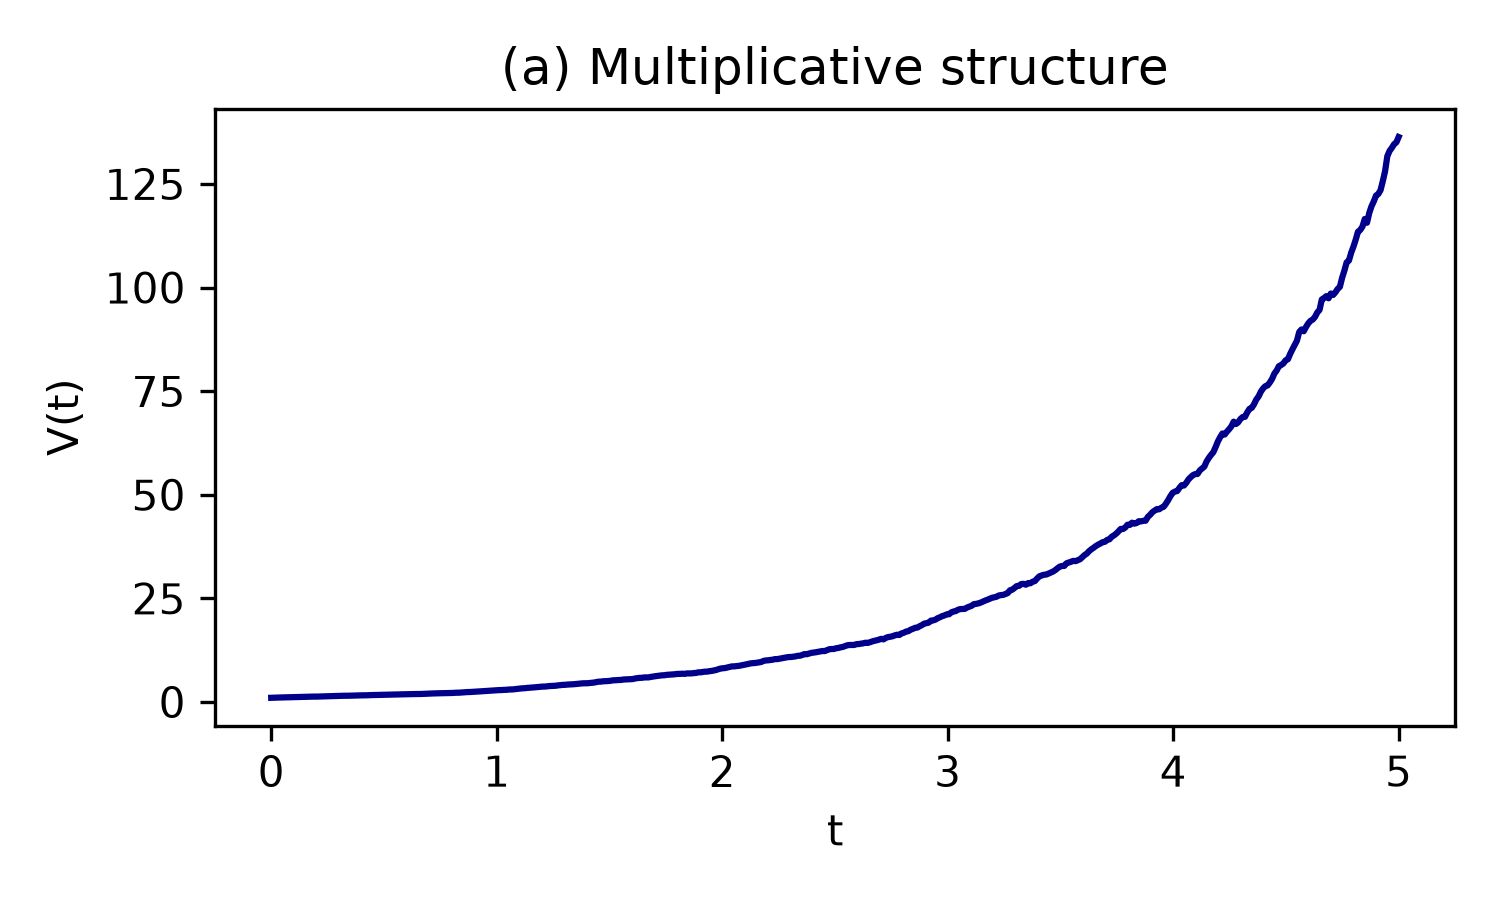
\includegraphics[width=\textwidth]{Python/figures/multiplicative_structure.png}
    \caption*{\textbf{(a) multiplicative：掛け算的悪化}\\外部ショックが企業価値に指数的に作用する構造}
\end{minipage}
\hfill
\begin{minipage}{0.33\textwidth}
    \centering
    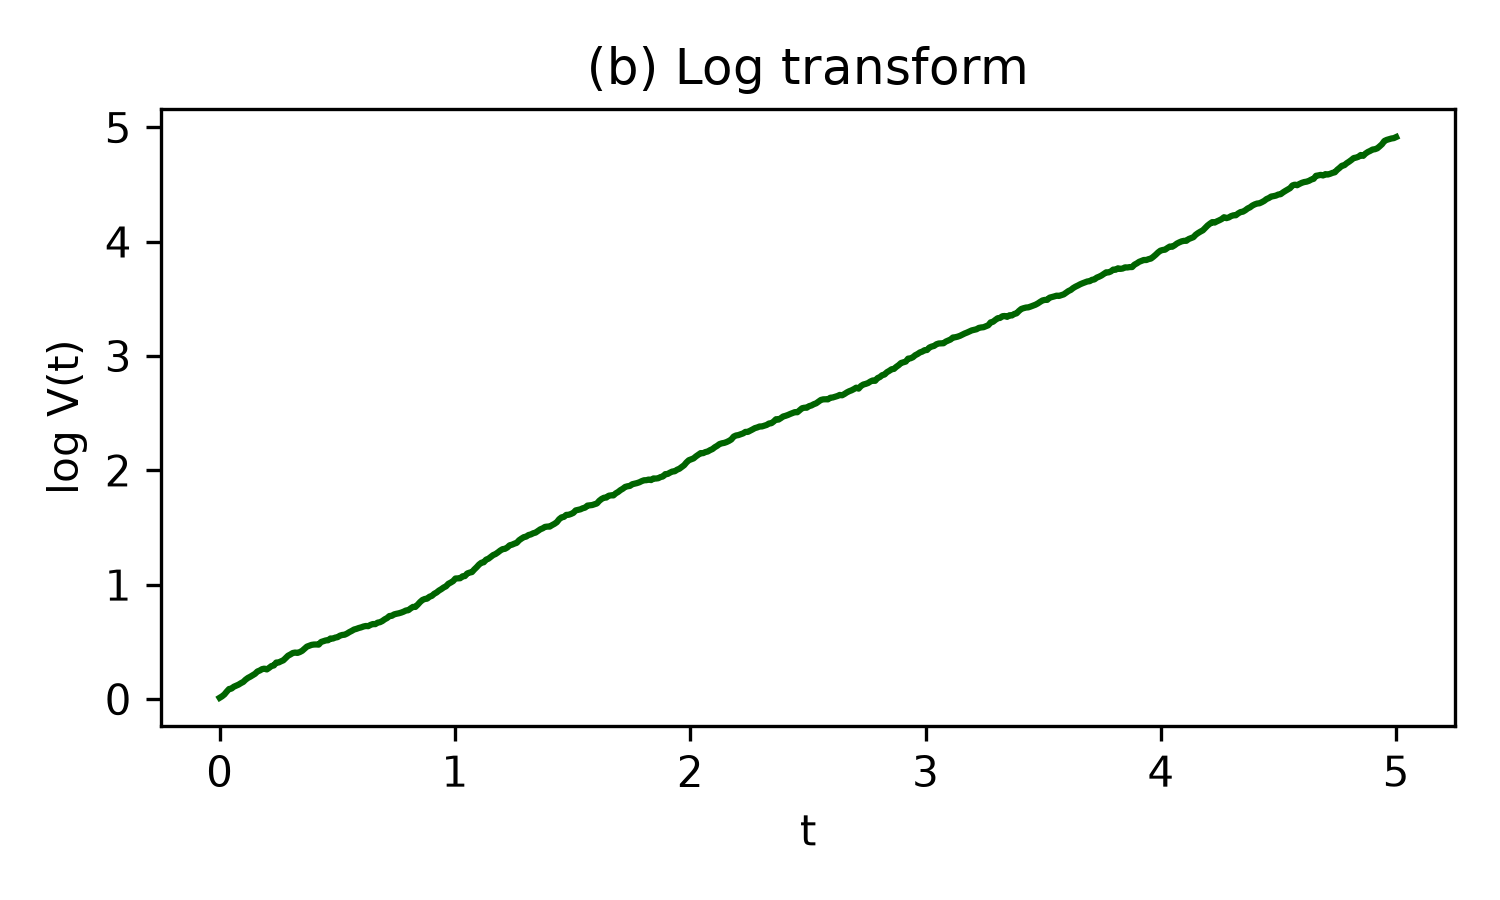
\includegraphics[width=\textwidth]{Python/figures/log_transform.png}
    \caption*{\textbf{(b) log：対数変換}\\multiplicative な変化が加法的（線形）に変換される}
\end{minipage}
\hfill
\begin{minipage}{0.33\textwidth}
    \centering
    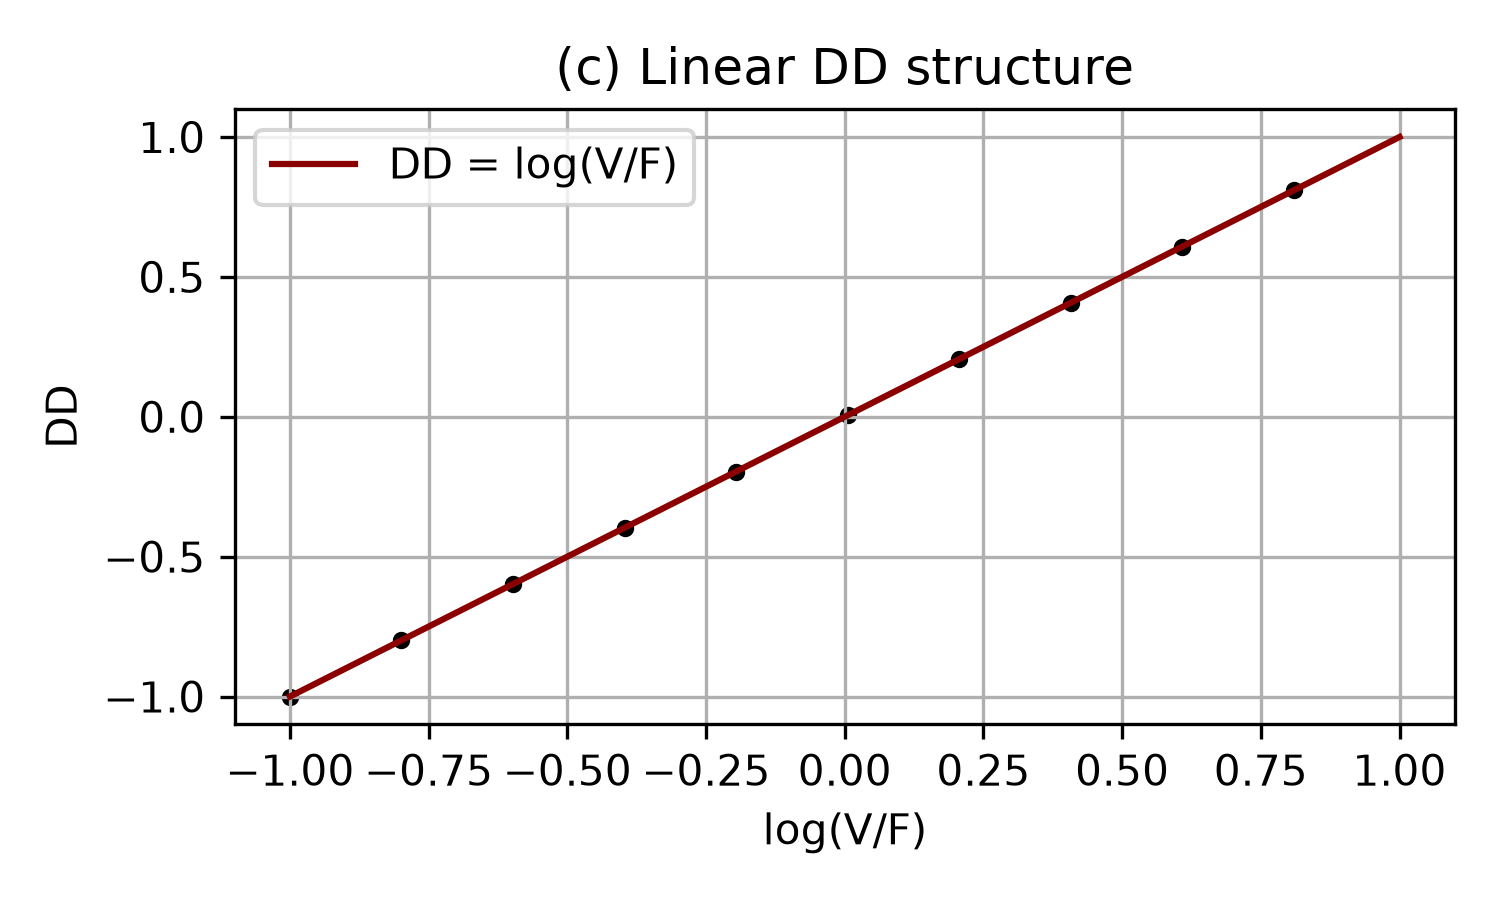
\includegraphics[width=\textwidth]{Python/figures/linear_dd.png}
    \caption*{\textbf{(c) linear：倒産距離 DD}\\閾値との差を線形距離として扱う構造}
\end{minipage}

\caption{multiplicative → log → linear の変換構造の概念図}
\label{fig:mult_log_linear}
\end{figure}

図 \ref{fig:mult_log_linear}は，企業価値の変動構造が「multiplicative（掛け算的）→ log（対数変換）→ linear（線形距離）」へと
段階的に変換される様子を概念的に示したものである。
(a) の multiplicative 構造では，外部ショックが企業価値に指数的に作用するため，
変動は時間とともに加速度的に拡大する。
(b) の log 変換では，multiplicative な変化が加法的な構造へと写像され，
企業価値の変動が線形的に扱えるようになる。
(c) の linear 構造では，倒産閾値との距離 $\log(V/F)$\footnote{
$\log(V/F)$ は Merton 型モデルにおける「倒産距離（distance to default）」の基本形であり，
企業価値 $V$ が倒産閾値 $F$（負債返済に必要な価値）からどれだけ離れているかを
対数比で測る指標である。
multiplicative（指数的）に変動する企業価値を log 変換することで，
倒産距離を加法的・線形的に扱えるようになる点が理論的な利点である。
}
が一次式として表現され，閾値との差を「線形距離」として評価できる点が
Merton 型モデルの基礎となる。

これら 3 つの図は，multiplicative な企業価値の変動が，
対数変換を経て線形な倒産距離として扱えることを視覚的に示している。


Bharath \& Shumway \parencite{BharathShumway2008} の proxy DD は，
その後の倒産研究において標準的手法として広く採用されている。
たとえば，Campbell, Hilscher \& Szilagyi \parencite{CampbellHilscherSzilagyi2008} は
市場要因と財務要因を統合した倒産モデルの中で proxy DD の有効性を示し，
Tinoco \& Wilson \parencite{TinocoWilson2013} はマクロショックと倒産距離の相互作用を実証した。
さらに Charalambakis \& Garrett \parencite{CharalambakisGarrett2019} は
産業特性を反映した倒産距離の再構築を行い，proxy DD の応用可能性を拡張している。


これらの研究は，B\&S の「機能形を維持しつつ観測可能な変数で倒産距離を構築する」
というアプローチが多様な産業・市場環境で有効であることを示している。
本研究もこの枠組みを踏まえ，新電力市場の制度的特徴に適合するよう
倒産構造を再構成する点に独自性がある。


% ---------------------------------------------
% Bharath & Shumway (2008) を採用する理論的必然性
% ---------------------------------------------

\vspace{1em}
\subsection{Bharath \& Shumway (2008) を採用する理論的必然性}

本研究が Bharath \& Shumway (2008)（以下 B\&S）を理論的基盤として採用する理由は，
新電力企業の倒産構造が Merton 型モデルの multiplicative な価値過程と整合的である一方で，
Merton モデルを直接推定することが実務的に困難であるためである。
Merton 型モデルは企業価値 $V_t$ が幾何ブラウン運動\footnote{
幾何ブラウン運動（Geometric Brownian Motion）とは、
企業価値が常に正の値をとり、ランダムに揺れながら指数的に変化する確率過程である。
本研究の視点では，この multiplicative な価値過程を前提とすることで，
企業価値の対数 $\log V_t$ が加法的（線形）な正規過程となり，
倒産閾値 $\log F$ との差 $\log(V_t/F)$ が「線形距離」として扱える点が重要となる。
この線形距離が Merton 型モデルにおける倒産距離（Distance to Default, DD）であり，
幾何ブラウン運動の仮定によって倒産確率が正規分布の累積分布として解析的に導出される。
}に従うという
multiplicative な構造を前提とし，倒産確率が次式で与えられる点に理論的な強みがある。



\[
P(\text{default}) = \Phi(-DD)
\]



この構造は，標準正規分布の図を用いることで直感的に理解できる。
図 \ref{fig:dd_normal} は，標準正規分布における倒産距離 $DD$ と
倒産確率 $\Phi(-DD)$ の関係を示している。
$DD$ が右方向に大きくなるほど，倒産確率に対応する左側の塗りつぶし部分が縮小し，
倒産確率が低下することが視覚的に理解できる。\footnote{
図では倒産確率 $\Phi(-DD)$ の定義に従い，横軸上の位置として
$-DD$ を描いている点に注意が必要である。
標準正規分布の左側の塗りつぶし部分は $\Phi(-DD)$ に対応するため，
図では「$-DD$ を左に動かすほど塗りつぶしが増える」ように見える。
しかしこれは符号の反転による見かけ上の挙動であり，
本質的には $DD$ が右方向に大きくなるほど $-DD$ は左に移動し，
結果として倒産確率 $\Phi(-DD)$ が減少する。
すなわち，図は $\Phi(-DD)$ の定義を忠実に描いているだけであり，
説明文の「$DD$ が大きいほど倒産確率が低い」という内容と
完全に整合している。
}


\begin{figure}[H]
\centering
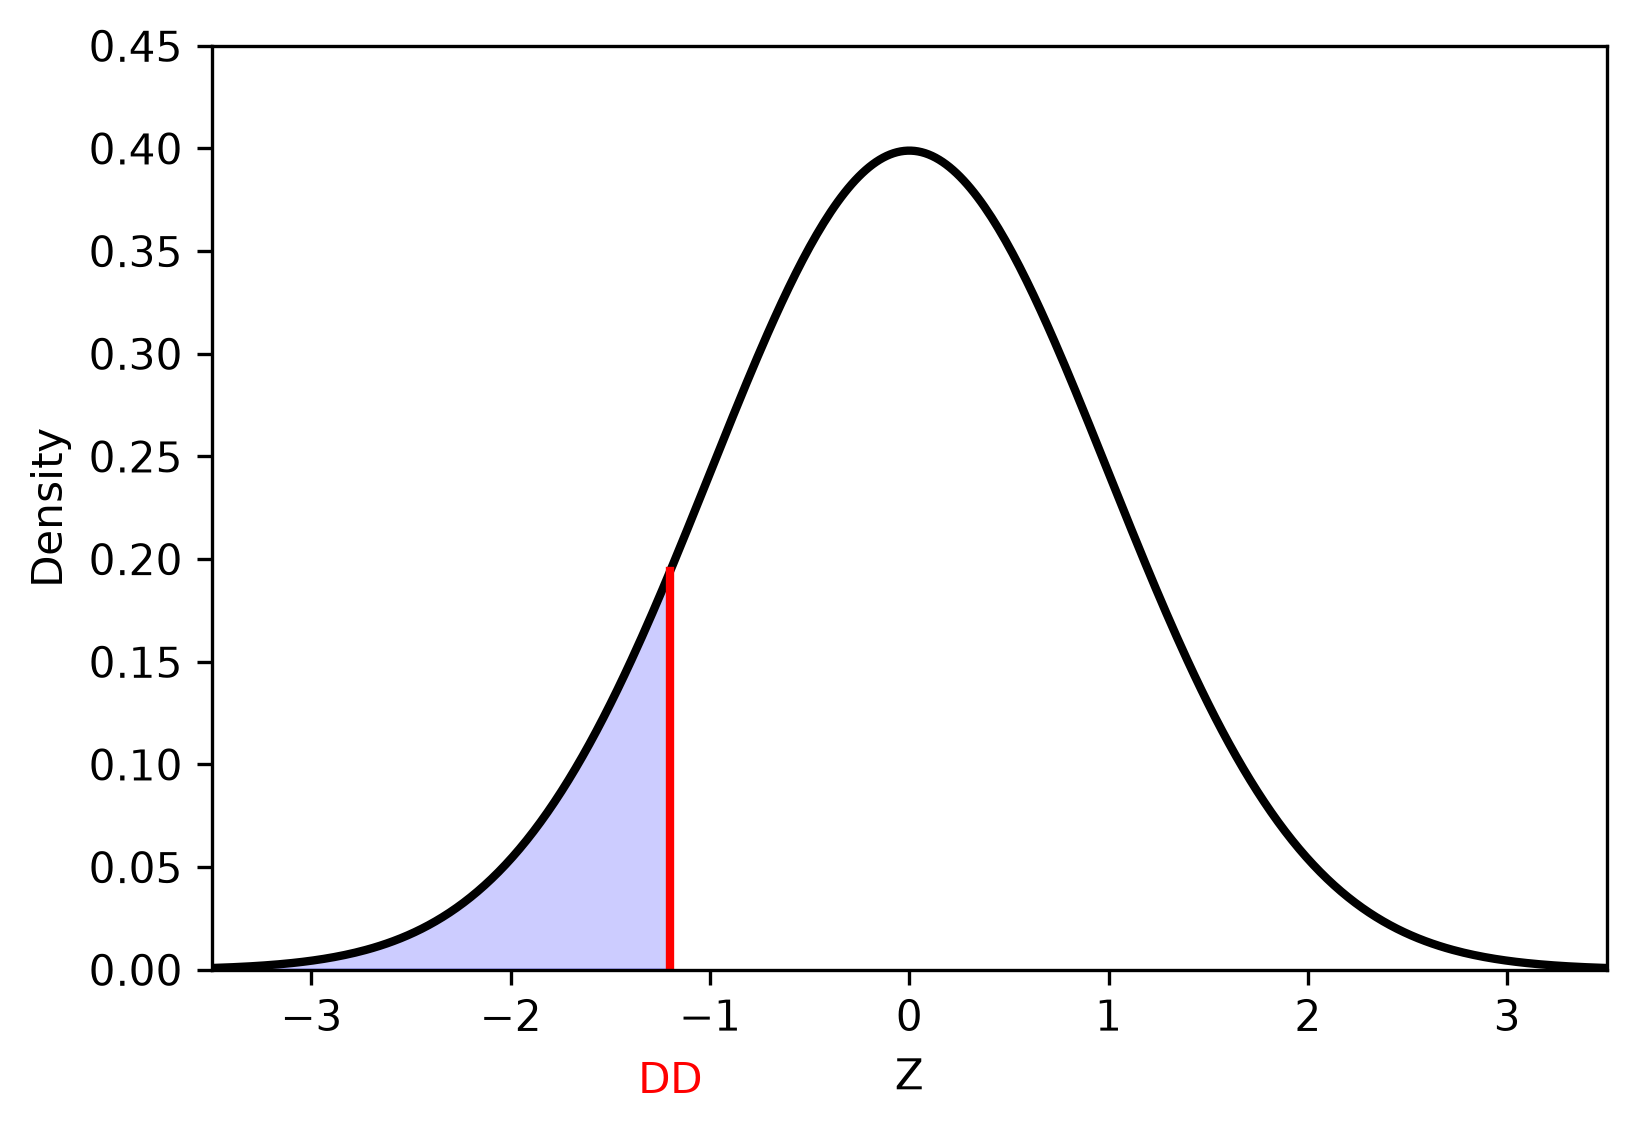
\includegraphics[width=0.85\textwidth]{figures/dd_normal.png}
\caption{標準正規分布における倒産距離 $DD$ と倒産確率 $\Phi(-DD)$}
\label{fig:dd_normal}
\end{figure}

B\&S は，この Merton 型モデルの multiplicative → log → linear の変換構造を維持しつつ，
倒産距離を観測可能な proxy によって線形化した点に独自性がある。
すなわち，Merton の理論的枠組みを損なうことなく，
倒産距離を回帰モデルで扱える形に変換した点に実務的価値がある。
この線形化の思想は，本研究が構築する四要素モデル
（収益性 $\mu$，外部ショック感応度 $\sigma$，支援能力 $S$，倒産閾値 $D$）
を実証的に検証するための理論的橋渡しとして機能する。

% ---------------------------------------------
% B&S を新電力に適用する際の前提修正の必要性
% ---------------------------------------------

\subsection{B\&S を新電力に適用する際の前提修正の必要性}

B\&S の枠組みは理論的に有効である一方で，新電力市場に適用するためには，
いくつかの前提条件を修正する必要がある。
第一に，B\&S は株価データを前提とするが，新電力企業の多くは非上場であり，
市場データを利用できない。
第二に，B\&S が想定する連続的な市場変動とは異なり，
新電力市場では JEPX 価格の急騰や制度変更など，
離散的かつ制度的ショックが倒産リスクを支配する。
第三に，B\&S の負債水準 $F$ は固定的であるのに対し，
新電力企業の倒産閾値 $D$ はインバランス料金や調達費用の変動により動的に変化する。
第四に，B\&S は親会社・自治体・金融機関による支援能力をモデルに含めていないが，
新電力企業において支援能力 $S$ は倒産リスクを大きく左右する要因である。

これらの点は B\&S の弱点ではなく，
むしろ新電力市場の制度的特殊性を反映した本研究独自の理論的貢献である\footnote{
ここで述べた前提修正は、B\&S の理論的限界を指摘するものではなく、
むしろ倒産モデルを新電力市場の制度構造に適合させるための
「構造的拡張（structural extension）」である。
すなわち、B\&S の基本枠組みを維持したまま、
市場特性に応じて倒産距離の構造要因を再定義することで、
モデルの適用範囲を拡張し、制度依存的な倒産メカニズムを
理論的に記述可能にする点に本研究の独自性がある。
この意味で、前提修正は B\&S の弱点の指摘ではなく、
新電力市場の制度的特徴を理論モデルに統合するための
学術的貢献として位置づけられる。
}
。
すなわち，本研究は B\&S の multiplicative → log → linear の構造を踏まえ，
新電力市場に特有の制度リスクを反映するために，
倒産距離の構造を四要素モデル（$\mu, \sigma, S, D$）として再構成する。
この再構成により，本研究の線形倒産距離 $Z_{\text{lin}}$ は，
B\&S の理論的系譜に属しながらも，
新電力企業の倒産メカニズムを説明するために必要な制度的要因を統合した
新たな倒産モデルとして位置づけられる。

% ---------------------------------------------
% 4.2 Merton モデル：multiplicative → log → linear の構造
% ---------------------------------------------
\section{Merton モデル：multiplicative → log → linear の構造}

本節では，Merton（1974）の構造モデルが前提とする
「multiplicative → log → linear」という価値過程の変換構造を整理し，
倒産距離（Distance to Default, DD）がどのように導出されるかを体系的に示す。
この変換構造は，企業価値の掛け算的な変動が対数変換によって線形化され，
倒産確率が標準正規分布の累積分布として表現できるという理論的特徴を持つ。

\subsection{multiplicative → log → linear の理論構造}

Merton（1974）の構造モデルは，企業価値 $V_t$ が幾何ブラウン運動に従うという
multiplicative な確率過程を前提とする点に特徴がある。企業価値のダイナミクス\footnote{
企業価値のダイナミクスとは，企業価値 $V_t$ が時間とともにどのように変化するかを記述する
確率的な運動法則を指す。Merton モデルではこの運動法則が幾何ブラウン運動として定式化され，
企業価値が掛け算的（multiplicative）に変動する構造を持つ。
この multiplicative な価値過程に対数変換を施すことで $\ln V_t$ が加法的（線形）な正規過程となり，
倒産閾値 $\ln F$ との差 $\log(V_t/F)$ が「線形距離」として扱えるようになる。
この線形距離が倒産距離（Distance to Default, DD）であり，
幾何ブラウン運動の仮定によって倒産確率が標準正規分布の累積分布
$\Phi(-DD)$ として解析的に導出される点が Merton 型モデルの理論的強みである。
}
は次式で与えられる：



\[
dV_t = \mu V_t\, dt + \sigma_V V_t\, dW_t
\]



ここで $\mu$ は企業価値の期待成長率，$\sigma_V$ は企業価値ボラティリティである。
multiplicative な価値過程に対数変換を施すと，加法的（線形）な構造へと写像される。

負債額 $F$ を倒産閾値とすると，1 年後の倒産距離（Distance to Default, DD）は



\[
DD = \frac{\ln(V/F) + (\mu - 0.5\sigma_V^2)}{\sigma_V}
\]



で表される\footnote{
この式の数学的導出（対数変換・正規分布化・閾値条件の整理）は付録Aに詳細を示している。
本文では概念構造に焦点を当てる。
}。これは倒産確率が



\[
\text{倒産確率} = f(\mu, \sigma_V, V/F)
\]



という multiplicative → log → linear の変換構造に基づいて決まることを示している。

倒産は「企業価値と負債の比率が確率的に閾値を下回るイベント」として定義され，
掛け算的なショックが対数変換を通じて線形化される点に理論的特徴がある\footnote{
倒産が「企業価値と負債の比率 $V/F$ が閾値を下回るイベント」として定義される理由は，
Merton 型モデルが企業価値 $V_t$ を基礎変数とし，負債額 $F$ を満期時点の返済義務として扱う
構造に基づく。満期時点において企業価値が負債額を下回れば倒産する。
この条件は $V_T < F$ と表され，対数変換によって $\log(V_T/F)$ が負になるかどうかという
「比率の閾値判定」に書き換えられる。さらに，$\log(V_T)$ が正規分布に従うことから，
$\log(V_T/F)$ は平均と分散をもつ線形距離として整理でき，その標準化が倒産距離
（Distance to Default, DD）となる。したがって，multiplicative → log → linear の変換構造は，
倒産イベント $V_T < F$ を「比率が閾値を下回る確率」として扱えるようにするための
数学的基盤である。
}。

\subsection{multiplicative → log → linear の変換構造が持つ大局的意味}

multiplicative → log → linear の構造は，倒産モデルにとって大局的な意味を持つ。
企業価値は外部ショックに対して掛け算的に反応するため，
multiplicative な価値過程を前提とすることは経済的にも数学的にも自然である。

さらに，multiplicative な構造は対数変換によって加法的（線形）に表現できるため，
複雑な相互作用を持つ倒産メカニズムを線形距離として扱うことが理論的に正当化される\footnote{
線形倒産距離として倒産メカニズムを扱うことは，Merton 型モデルの
multiplicative → log → linear の構造に基づき理論的に正当化されるだけでなく，
実証研究においても高い評価を得ている。Bharath \& Shumway（2008）は，
Merton の連続時間モデルを直接推定するよりも，観測可能な財務指標を用いた
線形倒産距離（proxy DD）が倒産予測の精度において優れていることを示した。
さらに Campbell, Hilscher \& Szilagyi（2008），Tinoco \& Wilson（2013），
Charalambakis \& Garrett（2019）など多くの後続研究が，
線形化された倒産距離が実務的・統計的に安定した予測性能を持つことを報告している。
このように，線形倒産距離は理論的整合性と実証的有効性の双方を備えた
倒産リスク指標として広く認められている。
}。

\subsection{Merton モデルにおける倒産距離の導出}

Merton モデルは連続時間の確率過程を前提としており，
企業価値 $V_t$ のダイナミクスを連続的に追跡し，
任意の時点 $T$ における倒産確率を理論的に導出する枠組みである。

対数変換を施すことで $\ln V_T$ が正規分布に従うことが示され，
倒産距離 $DD$ は平均と閾値の差を標準偏差で割った量として定義される：



\[
DD = \frac{\ln(V/F) + (\mu - 0.5\sigma_V^2)}{\sigma_V}
\]



倒産確率は標準正規分布の累積分布関数で表され，



\[
P(\text{default}) = \Phi(-DD)
\]



となる。倒産距離が大きいほど倒産確率は小さくなる。
倒産距離の導出過程（対数変換・正規分布化・閾値条件の整理）については，
詳細を付録Aに示している。

% ---------------------------------------------
% 4.3 Bharath \& Shumway (2008)：倒産距離の線形化と proxy 化
% ---------------------------------------------
\section{Bharath \& Shumway (2008)：倒産距離の線形化と proxy 化}

本節では，Merton モデルの理論構造（multiplicative → log → linear）を踏まえ，
その推定上の課題を解決するために Bharath \& Shumway（2008）（以下 B\&S）が提示した
離散時間モデルと proxy 化のアプローチを整理する。
Merton モデルは理論的に整合的である一方で，企業価値 $V$ や企業価値ボラティリティ
$\sigma_V$ が観測不可能であるため，連続時間モデルをそのまま推定することは
実務的に困難である。この問題意識が B\&S の出発点となった。

\subsection{連続時間モデルとしての Merton と，離散時間モデルとしての B\&S の相違}

Merton モデルは企業価値の連続的な変動を追跡し，任意時点の倒産確率を導出する
連続時間モデルである。しかし，企業価値 $V$ とそのボラティリティ $\sigma_V$ は
市場で直接観測できず，非線形方程式の同時推定が必要となるため，
実務的には不安定であることが知られている。

これに対して B\&S は，時間を離散化し，「1 年後に倒産するかどうか」という
固定された時間枠で倒産確率を推定する離散時間モデルを採用した。
すなわち，Merton の連続時間の数学的構造を捨てつつ，
multiplicative → log → linear の機能形のみを保持し，
観測可能な proxy を代入することで倒産距離を線形化した点に独自性がある。

この離散時間アプローチは，倒産が短期間に急激に顕在化する産業において
実務的にも理論的にも適合的であり，倒産予測モデルの実用性を大きく高めた。

\subsection{B\&S の naive predictor の理論的意義}

B\&S が提示した naive predictor\footnote{
Bharath \& Shumway（2008）が企業価値 $V$ や企業価値ボラティリティ $\sigma_V$ を
厳密に推定せず，観測可能な株式価値や負債額をそのまま代入して構築した
「素朴な（naive）倒産距離」を指す。
} は次式で与えられる：



\[
DD_{\text{naive}}
= \frac{\ln\left(\frac{E+F}{F}\right) + (\hat{\mu}-0.5\hat{\sigma}_V^2)}{\hat{\sigma}_V}
\]



ここで，
\begin{itemize}
    \item $\hat{\mu}$：株価リターン等から推定される収益性の proxy  
    \item $\hat{\sigma}_V$：株価ボラティリティから推定される企業価値ボラティリティの proxy  
\end{itemize}

この式は，Merton モデルの multiplicative → log → linear の構造を保持しつつ，
観測可能な proxy を代入することで推定可能性を確保したものである。
B\&S の重要な結論は「企業価値 $V$ と $\sigma_V$ の同時推定は必須ではない」という点にあり，
線形化された倒産距離が実務的に十分であることを示した。

\subsection{proxy 化の実務的意義と限界}

B\&S の proxy 化は倒産予測の実務に大きなインパクトを与えた\footnote{
Campbell, Hilscher \& Szilagyi（2008），Tinoco \& Wilson（2013），
Charalambakis \& Garrett（2019）など多くの後続研究が，
proxy DD が従来の財務指標よりも倒産予測精度に優れることを示している。
}。
株価データを用いることで，従来困難だった倒産距離の推定が可能となり，
信用リスク管理や企業モニタリングに広く応用された。

しかし，このアプローチには限界もある。

第一に，株価データを前提とするため非上場企業には適用困難である。  
第二に，市場ショックの連続性を前提とするが，新電力市場では離散的ショックが支配的である。  
第三に，負債水準を固定的に扱うが，新電力企業ではインバランス料金や調達費用により動的に変化する。  
第四に，支援能力をモデルに含めていないため，新電力企業特有の親会社・自治体・金融機関による
支援効果を捉えられない。

\subsection{B\&S の限界と，本研究における再構成の必要性}

以上の限界を踏まえ，本研究は B\&S の「proxy による線形化」という枠組みを土台とし，
新電力市場の制度的特徴を反映した四要素モデル
（収益性 $\mu$，外部ショック感応度 $\sigma$，支援能力 $S$，倒産閾値 $D$）
を構築し，線形倒産距離 $Z_{\text{lin}}$ として再定式化する。



\[
Z_{\text{lin}} = a\mu - b\sigma + cS - dD
\]



この $Z_{\text{lin}}$ は，Merton モデルの倒産距離および B\&S の proxy DD の機能形を継承しつつ，
新電力市場の制度的特徴を統合した新たな倒産モデルとして位置づけられる。

% ---------------------------------------------
% 4.4 本研究の線形倒産距離 $Z_{\text{lin}}$：新電力企業への写像
% ---------------------------------------------

\section{本研究の線形倒産距離 $Z_{\text{lin}}$：新電力企業への写像}

本節では，新電力企業の倒産メカニズムを構造的に整理し，
その主要因を観測可能な四要素（収益性 $\mu$，外部ショック感応度 $\sigma$，
支援能力 $S$，倒産閾値 $D$）として再構成したうえで，
これらを線形倒産距離 $Z_{\text{lin}}$ として形式化する。

新電力企業の倒産は，複数の要因が短期間に同時悪化することで急激に顕在化する。
既存の倒産事例（F-Power，エルピオ，ハルエネ等）では，
(i) 収益性の低下，(ii) 外部ショックへの脆弱性，
(iii) 支援能力の不足，(iv) 外部ショック時の支払義務の急増，
という四つの要因が繰り返し確認されており，
これらが倒産発生の主要因を網羅する「必要かつ十分な最小構成」であることが示されている。

この四要素はすべて観測可能な財務指標として定量化でき，
新電力企業の倒産メカニズムを構造的に捉えるうえで互いに独立である。
したがって，本研究はこれら四要素を倒産距離の構成要因として採用する。



\[
Z_{\text{lin}} = a\mu - b\sigma + cS - dD
\]



ここで，
\begin{itemize}
    \item $\mu$：収益性（営業利益率等）
    \item $\sigma$：外部ショック感応度（スポット依存度等）
    \item $S$：支援能力（親会社・自治体・金融機関）
    \item $D$：倒産閾値（外部ショック時の支払義務）
\end{itemize}

この $Z_{\text{lin}}$ は，数学的には四要素の線形結合であるが，
その背後には Merton モデルが前提とする
multiplicative → log → linear の構造が存在している。
すなわち，掛け算的に悪化する倒産要因を対数変換によって線形距離として扱うという
Merton 型モデルの機能形を保持しつつ，
観測可能な財務指標によって倒産距離を近似するという
Bharath \& Shumway（2008）の proxy 化の思想を継承している。

本研究の $Z_{\text{lin}}$ は，Merton → B\&S の理論的系譜に属しながら，
新電力市場の制度的特徴（支援能力の存在，動的な倒産閾値，離散的ショック）を統合した
新たな倒産距離として位置づけられる。

\begin{table}[H]
\centering
\caption{Merton → B\&S → 本研究の $Z_{\text{lin}}$ の対応関係}
\label{tab:merton_bs_zlin}

\renewcommand{\arraystretch}{1.4}
\begin{tabularx}{\textwidth}{p{0.22\textwidth} p{0.28\textwidth} X}
\toprule
\textbf{Merton (1974)} & \textbf{B\&S (2008)} & \textbf{本研究の $Z_{\text{lin}}$} \\
\midrule

$\mu$（企業価値の期待成長率） &
過去リターン等で proxy &
収益性（営業利益率） \\

$\sigma_V$（企業価値ボラティリティ） &
株価ボラティリティで proxy &
外部ショック感応度（スポット依存度） \\

$F$（負債額） &
帳簿価値で proxy &
倒産閾値 $D$（外部ショック時の支払義務） \\

--- & --- &
支援能力 $S$（外生的緩和要因） \\

\midrule

倒産距離 $DD$ &
naive DD（proxy DD） &
$Z_{\text{lin}}$（線形倒産距離） \\

\bottomrule
\end{tabularx}
\end{table}

以上より，$Z_{\text{lin}}$ は

\begin{quote}
Merton モデルの倒産距離を B\&S の proxy 化の思想に基づき線形化し，
新電力企業の制度的特徴を反映するよう再構築した潜在倒産距離
\end{quote}

として理論的に位置づけられる。

次章では，この $Z_{\text{lin}}$ を Ordered Logit モデルに接続し，
新電力企業の倒産ステージ（Active → Administration → Liquidation → Dissolved）へと
離散的に写像することで，実証分析を行う。

% ---------------------------------------------
% 4.5 連続的倒産距離 $Z_{\text{lin}}$ と Ordered Logit の接続
% ---------------------------------------------

\section{連続的倒産距離 $Z_{\text{lin}}$ と Ordered Logit の接続}

前節で導出した線形倒産距離 $Z_{\text{lin}}$\footnote{
潜在変数（latent index）を $Z$ と表記するのは計量経済学の慣例であり，
特別な理論的意味を持つわけではない。
} は，新電力企業の倒産リスクを連続的な尺度として表す潜在倒産距離である。
しかし，実際の倒産データは連続量として観測されるわけではなく，
企業はある時点で「存続」「財務悪化」「撤退・吸収合併」「法的倒産」といった
離散的なステージに分類される。

したがって，連続的倒産距離 $Z_{\text{lin}}$ を実証分析で扱うためには，
連続量を離散カテゴリへ写像する確率構造が必要となる。
この橋渡しを行う標準的な枠組みが Ordered Logit モデルである。

\subsection{Ordered Logit モデルの潜在変数構造}

Ordered Logit モデルは，倒産の背後に連続的な潜在変数 $y^*_{i,t}$ が存在すると仮定し，
その値が複数の閾値（cutpoints）$\tau_1, \tau_2, \tau_3$ をどこまで超えるかによって，
離散的な倒産ステージが決定されるという構造を持つ。

潜在変数は次式で表される：

\begin{equation}
y^*_{i,t}
=
\beta_1 D_{i,t}
+ \beta_2 \mu_{i,t}
+ \beta_3 \sigma_{i,t}
+ \beta_4 S_{i,t}
+ \varepsilon_{i,t},
\qquad
\varepsilon_{i,t} \sim \text{Logistic}(0,1)
\label{eq:latent_y_appendix}
\end{equation}

式 \eqref{eq:latent_y_appendix} の線形部分 $X_{i,t}\beta$ は，
第4章で導出した線形倒産距離



\[
Z_{\text{lin}} = a\mu - b\sigma + cS - dD
\]



と構造的に一致している。
すなわち，$Z_{\text{lin}}$ を Ordered Logit の潜在変数 $y^*$ に写像することで，
理論モデル（連続的倒産距離）と実証モデル（離散的倒産ステージ）が
自然に接続される。

\subsection{cutpoint（閾値）の推定と離散カテゴリへの写像}

Ordered Logit モデルにおける cutpoint（閾値）$\tau_k$ は，
研究者が任意に設定する境界ではなく，
ロジット係数 $\beta$ と同様に尤度最大化（MLE）によって
データから推定される内生的パラメータである。
この性質により，潜在変数の連続スケールをどのように区切るべきかを
モデル自身がデータから学習することが可能となり，
倒産ステージの境界を恣意的に設定する必要がない。

\subsection{本研究における Ordered Logit の役割}

以上より，Ordered Logit モデルは，
第4章で導出した連続的倒産距離 $Z_{\text{lin}}$ を，
実証分析で扱う離散的倒産ステージへと変換するための
数学的に整合的な枠組みである。

次章では，この Ordered Logit モデルを用いて，
日本企業および英国企業の倒産ステージを推定し，
四要素モデル（$\mu, \sigma, S, D$）が倒産リスクをどのように規定するかを
実証的に検証する。

% ---------------------------------------------
% 4.6 Bharath \& Shumway (2008) と本研究の比較
% ---------------------------------------------

\section{Bharath \& Shumway (2008) と本研究の比較}
\label{sec:bs_comparison}

本節では，Bharath \& Shumway（2008）（以下 B\&S）が提示した
proxy 化による倒産距離と，本研究が構築した線形倒産距離
$Z_{\text{lin}}$ の関係を整理し，両者の共通点と相違点を明確化する。

B\&S は，Merton モデルの連続時間構造を直接推定するのではなく，
multiplicative → log → linear の機能形を保持したまま，
観測可能な財務指標を代入することで倒産距離を線形化した。
この「機能形を維持しつつ観測可能な変数で倒産距離を構築する」という
アプローチは，その後の倒産研究において標準的手法として広く採用されている。
たとえば Campbell, Hilscher \& Szilagyi (2008) は市場要因と財務要因を統合した
倒産モデルの中で proxy DD の有効性を示し，
Tinoco \& Wilson (2013) はマクロショックと倒産距離の相互作用を実証した。
さらに Charalambakis \& Garrett (2019) は産業特性を反映した倒産距離の再構築を行い，
proxy DD の応用可能性を拡張している。

本研究はこの B\&S の枠組みを継承しつつ，
新電力市場の制度的特徴（離散的ショック，動的な倒産閾値，支援能力の存在）を
反映するために倒産距離を再構成した。
すなわち，収益性 $\mu$，外部ショック感応度 $\sigma$，
支援能力 $S$，倒産閾値 $D$ の四要素を観測可能変数として導入し，
新電力企業の倒産メカニズムに適合する線形倒産距離
$Z_{\text{lin}}$ を構築した点に独自性がある。

以下では，B\&S と本研究の線形倒産距離の対応関係を整理する。

\begin{table}[H]
\centering
\caption{Bharath \& Shumway (2008) と本研究の比較}
\label{tab:bs_vs_this}

\renewcommand{\arraystretch}{1.4}
\begin{tabularx}{\textwidth}{p{0.28\textwidth} p{0.30\textwidth} X}
\toprule
\textbf{項目} & \textbf{Bharath \& Shumway (2008)} & \textbf{本研究（新電力倒産モデル）} \\
\midrule

理論的基盤 &
Merton 型モデルの倒産距離を proxy 化 &
Merton/B\&S の構造を新電力の制度構造に写像し再構成 \\

倒産距離の構造 &
$\mu$, $\sigma_V$, $V/F$ に基づく線形倒産距離 &
収益性 $\mu$, 外部ショック感応度 $\sigma$, 支援能力 $S$, 倒産閾値 $D$ に基づく線形倒産距離 $Z_{\text{lin}}$ \\

扱うリスク要因 &
市場リスク・財務リスク（株価データ中心） &
外部ショック（JEPX 価格・制度コスト），支援能力，倒産閾値の変動など新電力特有の制度的リスク \\

目的 &
企業価値モデルの proxy 化と倒産予測精度の向上 &
新電力市場に特有の倒産構造の理論的解明と倒産距離の再構築 \\

独自性 &
Merton の機能形を維持した proxy DD の提案 &
四要素モデル（$\mu, \sigma, S, D$）を用いた新電力特有の倒産距離の構築 \\

\bottomrule
\end{tabularx}
\end{table}

以上より，本研究の $Z_{\text{lin}}$ は，
B\&S の理論的系譜に属しながらも，
新電力企業の倒産メカニズムを説明するために必要な制度的要因を統合した
新たな倒産距離として位置づけられる。
